% ==========================================
% CHAPTER 5: EXPERIMENTS & RESULTS
% ==========================================
\chapter{Experiments and Results}
\label{chap:experiments}

This chapter presents the empirical validation of the KinetoCheck framework through quantitative and qualitative analyses. It documents the experimental setup, reports performance metrics comparing baseline, phase-aware, and ROM-regularized variants, and provides ablation studies to isolate the contribution of each architectural component.

\section{Experimental Setup and Protocol}
The experiments reported in this chapter follow the subject-wise split protocol described in Chapter 4, where subjects are assigned to non-overlapping train, validation, and test sets. To validate strict generalization under more demanding conditions, Leave-One-Subject-Out (LOSO) evaluation is also performed as noted below.

\subsection{Dataset Characteristics}
The UI-PRMD dataset contains 1,980 sequences across 10 subjects and 10 exercises, with a balanced distribution of correct and incorrect executions. Each subject performs each exercise multiple times, resulting in a rich set of movement variations. The dataset is captured using a Vicon motion capture system, providing high-fidelity 3D joint coordinates. The 39-joint Vicon captures are mapped to a 17-joint representation consistent with MediaPipe’s output, as illustrated in Figure~\ref{fig:vicon-comparison}.

\begin{figure}[H]
    \centering
    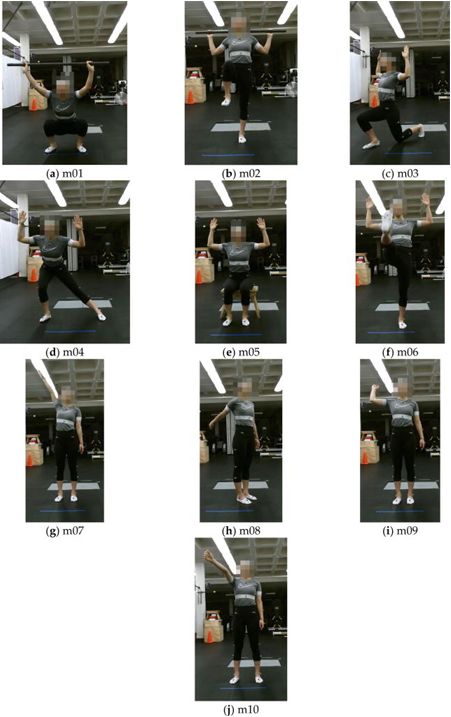
\includegraphics[width=0.75\textwidth]{figures/uiprmd_exercises.png}
    \caption{UI-PRMD exercises visualization. \cite{VJPB18}}
    \label{fig:uiprmd-visualization}
\end{figure}

\begin{table}[htbp]
\centering
\small
\setlength{\tabcolsep}{5pt}
\renewcommand{\arraystretch}{1.15}

\begin{tabularx}{\textwidth}{|>{\centering\arraybackslash}p{1.4cm}|>{\raggedright\arraybackslash}X|>{\centering\arraybackslash}p{2.3cm}|>{\centering\arraybackslash}p{2.6cm}|>{\centering\arraybackslash}p{2.0cm}|}
\hline
Exercise ID & Exercise Name & Correct Count & Incorrect Count & Total Count \\
\hline
1 & exercise\_01 & 110 & 110 & 220 \\
2 & exercise\_02 & 110 & 110 & 220 \\
3 & exercise\_03 & 99 & 99 & 198 \\
4 & exercise\_04 & 110 & 110 & 220 \\
5 & exercise\_05 & 110 & 110 & 220 \\
6 & exercise\_06 & 110 & 110 & 220 \\
7 & exercise\_07 & 110 & 110 & 220 \\
8 & exercise\_08 & 110 & 110 & 220 \\
9 & exercise\_09 & 110 & 110 & 220 \\
10 & exercise\_10 & 110 & 110 & 220 \\
\hline
\end{tabularx}
\caption{Dataset composition by exercise and label}
\label{tab:T1}
\end{table}


\begin{figure}[H]
    \centering
    \begin{minipage}[t]{0.48\textwidth}
        \centering
        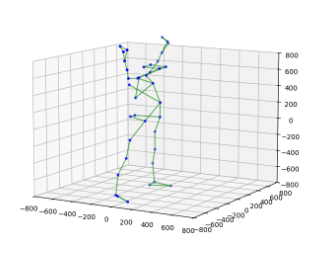
\includegraphics[width=\linewidth]{figures/VICON-39-joints-exercise0-frame-3d-plot.png}
        \vspace{0.2cm}
        \small (a) Full 39-joint Vicon capture
    \end{minipage}
    \hfill
    \begin{minipage}[t]{0.48\textwidth}
        \centering
        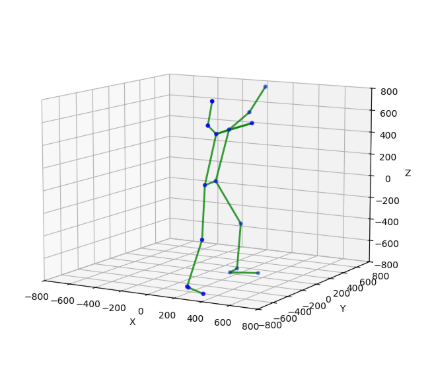
\includegraphics[width=\linewidth]{figures/VICON-17-COCO-joints-exercise0-frame-3d-plot.png}
        \vspace{0.2cm}
        \small (b) Mapped 17-joint representation
    \end{minipage}
    \vspace{0.4cm}
    \caption{Example 3D Vicon captures showing the original marker-rich representation and the reduced 17-joint representation used in the thesis pipeline.}
    \label{fig:vicon-comparison}
\end{figure}

\section{Quantitative Analysis}
The quantitative analysis evaluates the framework across four distinct training configurations to isolate the impact of each architectural component. We report standard categorical metrics (accuracy, precision, recall, and F1-score) to evaluate binary correctness decisions, alongside the automatically calibrated decision threshold for each exercise. 

Because the Siamese network architecture regresses a continuous similarity score rather than predicting a discrete class label, the \textbf{threshold} serves as the explicit decision boundary. If a patient's execution score meets or exceeds this calibrated value, the movement is classified as correct. Notably, this boundary is dynamically calibrated during the validation phase to maximize the F1-score, accommodating the unique biomechanical variance and baseline difficulty inherent to each specific exercise.

To rigorously test the system's capabilities and generalization, the evaluation is broken down into the following configurations:
\begin{itemize}
    \item \textbf{Baseline Variant} (Table \ref{tab:baseline}): The standard Siamese ST-GAT architecture without auxiliary temporal alignment or spatial penalties.
    \item \textbf{Phase-Aware Variant without ROM} (Table \ref{tab:phase-aware-no-rom}): Introduces the temporal phase-alignment module to synchronize varying execution speeds.
    \item \textbf{Phase-Aware Variant with ROM} (Table \ref{tab:phase-aware-rom}): Adds Range-of-Motion regularization to explicitly penalize partial-range executions.
    \item \textbf{Leave-One-Subject-Out (LOSO)} (Table \ref{tab:loso-metrics}): Applies the most robust configuration (Phase-Aware with ROM) under strict cross-subject validation to test true generalization against entirely unseen patients.
\end{itemize}

\begin{table}[htbp]
    \centering
    \caption{Baseline variant.}
    \label{tab:baseline}
    \begin{tabularx}{0.8\textwidth}{@{} c c c c c c @{}}
        \toprule
        \textbf{Ex. ID} & \textbf{Threshold} & \textbf{Accuracy} & \textbf{Precision} & \textbf{Recall} & \textbf{F1} \\
        \midrule
        1  & -0.415 & 0.850 & 0.769 & 1.000 & 0.870 \\
        2  &  0.952 & 1.000 & 1.000 & 1.000 & 1.000 \\
        3  & -0.199 & 1.000 & 1.000 & 1.000 & 1.000 \\
        4  &  0.481 & 0.800 & 0.714 & 1.000 & 0.833 \\
        5  & -0.506 & 1.000 & 1.000 & 1.000 & 1.000 \\
        6  &  0.663 & 0.950 & 0.909 & 1.000 & 0.952 \\
        7  &  0.793 & 0.900 & 1.000 & 0.800 & 0.889 \\
        8  & -0.255 & 1.000 & 1.000 & 1.000 & 1.000 \\
        9  &  0.990 & 0.800 & 0.750 & 0.900 & 0.818 \\
        10 &  0.924 & 1.000 & 1.000 & 1.000 & 1.000 \\
        \bottomrule
    \end{tabularx}
\end{table}

\begin{table}[htbp]
    \centering
    \caption{Phase-aware variant without ROM regularization.}
    \label{tab:phase-aware-no-rom}
    \begin{tabularx}{0.8\textwidth}{@{} c c c c c c @{}}
        \toprule
        \textbf{Ex. ID} & \textbf{Threshold} & \textbf{Accuracy} & \textbf{Precision} & \textbf{Recall} & \textbf{F1} \\
        \midrule
        1  &  0.758 & 1.000 & 1.000 & 1.000 & 1.000 \\
        2  &  0.822 & 1.000 & 1.000 & 1.000 & 1.000 \\
        3  & -0.151 & 0.900 & 0.900 & 0.900 & 0.900 \\
        4  &  0.864 & 0.900 & 0.833 & 1.000 & 0.909 \\
        5  & -0.539 & 0.900 & 0.833 & 1.000 & 0.909 \\
        6  &  0.697 & 0.950 & 0.909 & 1.000 & 0.952 \\
        7  &  0.956 & 1.000 & 1.000 & 1.000 & 1.000 \\
        8  &  0.601 & 1.000 & 1.000 & 1.000 & 1.000 \\
        9  &  0.754 & 0.500 & 0.500 & 1.000 & 0.667 \\
        10 &  0.880 & 1.000 & 1.000 & 1.000 & 1.000 \\
        \bottomrule
    \end{tabularx}
\end{table}

\begin{table}[htbp]
    \centering
    \caption{Phase-aware variant with ROM (Range-of-Motion) regularization.}
    \label{tab:phase-aware-rom}
    \begin{tabularx}{0.8\textwidth}{@{} c c c c c c @{}}
        \toprule
        \textbf{Ex. ID} & \textbf{Threshold} & \textbf{Accuracy} & \textbf{Precision} & \textbf{Recall} & \textbf{F1} \\
        \midrule
        1  &  0.886 & 0.900 & 0.833 & 1.000 & 0.909 \\
        2  &  0.060 & 1.000 & 1.000 & 1.000 & 1.000 \\
        3  &  0.233 & 0.850 & 1.000 & 0.700 & 0.824 \\
        4  &  0.801 & 0.900 & 0.833 & 1.000 & 0.909 \\
        5  & -0.663 & 0.950 & 0.909 & 1.000 & 0.952 \\
        6  &  0.027 & 0.850 & 0.818 & 0.900 & 0.857 \\
        7  & -0.387 & 1.000 & 1.000 & 1.000 & 1.000 \\
        8  & -0.552 & 0.600 & 0.556 & 1.000 & 0.714 \\
        9  &  0.445 & 0.800 & 0.714 & 1.000 & 0.833 \\
        10 &  0.990 & 1.000 & 1.000 & 1.000 & 1.000 \\
        \bottomrule
    \end{tabularx}
\end{table}

\begin{table}[htbp]
    \centering
    \caption{Leave-One-Subject-Out (LOSO) Aggregated Metrics per Exercise. Evaluated utilizing the Phase-Aware variant with ROM regularization.}
    \label{tab:loso-metrics}
    \begin{tabularx}{0.8\textwidth}{@{} c c c c c c @{}}
        \toprule
        \textbf{Ex. ID} & \textbf{Threshold} & \textbf{Accuracy} & \textbf{Precision} & \textbf{Recall} & \textbf{F1} \\
        \midrule
        1  &  0.532 & 0.865 & 0.816 & 1.000 & 0.891 \\
        2  &  0.506 & 0.945 & 0.914 & 1.000 & 0.951 \\
        3  &  0.645 & 0.755 & 0.724 & 0.988 & 0.821 \\
        4  &  0.602 & 0.760 & 0.705 & 0.990 & 0.814 \\
        5  &  0.365 & 0.910 & 0.881 & 0.960 & 0.916 \\
        6  &  0.499 & 0.965 & 0.949 & 0.990 & 0.968 \\
        7  &  0.423 & 0.920 & 0.890 & 1.000 & 0.935 \\
        8  &  0.819 & 0.800 & 0.772 & 1.000 & 0.856 \\
        9  &  0.505 & 0.830 & 0.803 & 0.990 & 0.872 \\
        10 &  0.596 & 0.795 & 0.750 & 0.990 & 0.844 \\
        \bottomrule
    \end{tabularx}
\end{table}

While the aggregated metrics across the subject-wise splits (Tables \ref{tab:baseline} -- \ref{tab:phase-aware-rom}) show high initial performance, a granular analysis reveals the critical importance of the architectural enhancements. Specifically, the baseline model frequently struggles to accurately assess videos containing partial-range executions, where a patient maintains correct anatomical posture but prematurely terminates the repetition. 

The introduction of the phase-aware variant, specifically coupled with ROM regularization, explicitly addresses this clinical nuance. By actively penalizing incomplete spatial trajectories, the ROM-regularized model significantly reduces false positives. In a real-world rehabilitation context, this behavior is paramount to ensure patients are not incorrectly rewarded for incomplete routines.

Furthermore, Table \ref{tab:loso-metrics} validates the true generalizability of the framework. Evaluated under strict Leave-One-Subject-Out (LOSO) conditions—which prevents the network from memorizing patient-specific physical traits—the metrics naturally exhibit a slight, expected decrease compared to standard splits. However, maintaining high average F1-scores across entirely unseen subjects confirms that the network has successfully learned to generalize underlying biomechanical movement patterns, effectively solving the identity leakage problem.\section{Quantitative Analysis}
The quantitative analysis evaluates the framework across four distinct training configurations to isolate the impact of each architectural component. We report standard categorical metrics (accuracy, precision, recall, and F1-score) to evaluate binary correctness decisions, alongside the automatically calibrated decision threshold for each exercise. 

Because the Siamese network architecture regresses a continuous similarity score rather than predicting a discrete class label, the \textbf{threshold} serves as the explicit decision boundary. If a patient's execution score meets or exceeds this calibrated value, the movement is classified as correct. Notably, this boundary is dynamically calibrated during the validation phase to maximize the F1-score, accommodating the unique biomechanical variance and baseline difficulty inherent to each specific exercise.

To rigorously test the system's capabilities and generalization, the evaluation is broken down into the following configurations:
\begin{itemize}
    \item \textbf{Baseline Variant} (Table \ref{tab:baseline}): The standard Siamese ST-GAT architecture without auxiliary temporal alignment or spatial penalties.
    \item \textbf{Phase-Aware Variant without ROM} (Table \ref{tab:phase-aware-no-rom}): Introduces the temporal phase-alignment module to synchronize varying execution speeds.
    \item \textbf{Phase-Aware Variant with ROM} (Table \ref{tab:phase-aware-rom}): Adds Range-of-Motion regularization to explicitly penalize partial-range executions.
    \item \textbf{Leave-One-Subject-Out (LOSO)} (Table \ref{tab:loso-metrics}): Applies the most robust configuration (Phase-Aware with ROM) under strict cross-subject validation to test true generalization against entirely unseen patients.
\end{itemize}

\begin{table}[htbp]
    \centering
    \caption{Baseline variant.}
    \label{tab:baseline}
    \begin{tabularx}{0.8\textwidth}{@{} c c c c c c @{}}
        \toprule
        \textbf{Ex. ID} & \textbf{Threshold} & \textbf{Accuracy} & \textbf{Precision} & \textbf{Recall} & \textbf{F1} \\
        \midrule
        1  & -0.415 & 0.850 & 0.769 & 1.000 & 0.870 \\
        2  &  0.952 & 1.000 & 1.000 & 1.000 & 1.000 \\
        3  & -0.199 & 1.000 & 1.000 & 1.000 & 1.000 \\
        4  &  0.481 & 0.800 & 0.714 & 1.000 & 0.833 \\
        5  & -0.506 & 1.000 & 1.000 & 1.000 & 1.000 \\
        6  &  0.663 & 0.950 & 0.909 & 1.000 & 0.952 \\
        7  &  0.793 & 0.900 & 1.000 & 0.800 & 0.889 \\
        8  & -0.255 & 1.000 & 1.000 & 1.000 & 1.000 \\
        9  &  0.990 & 0.800 & 0.750 & 0.900 & 0.818 \\
        10 &  0.924 & 1.000 & 1.000 & 1.000 & 1.000 \\
        \bottomrule
    \end{tabularx}
\end{table}

\begin{table}[htbp]
    \centering
    \caption{Phase-aware variant without ROM regularization.}
    \label{tab:phase-aware-no-rom}
    \begin{tabularx}{0.8\textwidth}{@{} c c c c c c @{}}
        \toprule
        \textbf{Ex. ID} & \textbf{Threshold} & \textbf{Accuracy} & \textbf{Precision} & \textbf{Recall} & \textbf{F1} \\
        \midrule
        1  &  0.758 & 1.000 & 1.000 & 1.000 & 1.000 \\
        2  &  0.822 & 1.000 & 1.000 & 1.000 & 1.000 \\
        3  & -0.151 & 0.900 & 0.900 & 0.900 & 0.900 \\
        4  &  0.864 & 0.900 & 0.833 & 1.000 & 0.909 \\
        5  & -0.539 & 0.900 & 0.833 & 1.000 & 0.909 \\
        6  &  0.697 & 0.950 & 0.909 & 1.000 & 0.952 \\
        7  &  0.956 & 1.000 & 1.000 & 1.000 & 1.000 \\
        8  &  0.601 & 1.000 & 1.000 & 1.000 & 1.000 \\
        9  &  0.754 & 0.500 & 0.500 & 1.000 & 0.667 \\
        10 &  0.880 & 1.000 & 1.000 & 1.000 & 1.000 \\
        \bottomrule
    \end{tabularx}
\end{table}

\begin{table}[htbp]
    \centering
    \caption{Phase-aware variant with ROM (Range-of-Motion) regularization.}
    \label{tab:phase-aware-rom}
    \begin{tabularx}{0.8\textwidth}{@{} c c c c c c @{}}
        \toprule
        \textbf{Ex. ID} & \textbf{Threshold} & \textbf{Accuracy} & \textbf{Precision} & \textbf{Recall} & \textbf{F1} \\
        \midrule
        1  &  0.886 & 0.900 & 0.833 & 1.000 & 0.909 \\
        2  &  0.060 & 1.000 & 1.000 & 1.000 & 1.000 \\
        3  &  0.233 & 0.850 & 1.000 & 0.700 & 0.824 \\
        4  &  0.801 & 0.900 & 0.833 & 1.000 & 0.909 \\
        5  & -0.663 & 0.950 & 0.909 & 1.000 & 0.952 \\
        6  &  0.027 & 0.850 & 0.818 & 0.900 & 0.857 \\
        7  & -0.387 & 1.000 & 1.000 & 1.000 & 1.000 \\
        8  & -0.552 & 0.600 & 0.556 & 1.000 & 0.714 \\
        9  &  0.445 & 0.800 & 0.714 & 1.000 & 0.833 \\
        10 &  0.990 & 1.000 & 1.000 & 1.000 & 1.000 \\
        \bottomrule
    \end{tabularx}
\end{table}

\begin{table}[htbp]
    \centering
    \caption{Leave-One-Subject-Out (LOSO) Aggregated Metrics per Exercise. Evaluated utilizing the Phase-Aware variant with ROM regularization.}
    \label{tab:loso-metrics}
    \begin{tabularx}{0.8\textwidth}{@{} c c c c c c @{}}
        \toprule
        \textbf{Ex. ID} & \textbf{Threshold} & \textbf{Accuracy} & \textbf{Precision} & \textbf{Recall} & \textbf{F1} \\
        \midrule
        1  &  0.532 & 0.865 & 0.816 & 1.000 & 0.891 \\
        2  &  0.506 & 0.945 & 0.914 & 1.000 & 0.951 \\
        3  &  0.645 & 0.755 & 0.724 & 0.988 & 0.821 \\
        4  &  0.602 & 0.760 & 0.705 & 0.990 & 0.814 \\
        5  &  0.365 & 0.910 & 0.881 & 0.960 & 0.916 \\
        6  &  0.499 & 0.965 & 0.949 & 0.990 & 0.968 \\
        7  &  0.423 & 0.920 & 0.890 & 1.000 & 0.935 \\
        8  &  0.819 & 0.800 & 0.772 & 1.000 & 0.856 \\
        9  &  0.505 & 0.830 & 0.803 & 0.990 & 0.872 \\
        10 &  0.596 & 0.795 & 0.750 & 0.990 & 0.844 \\
        \bottomrule
    \end{tabularx}
\end{table}

While the aggregated metrics across the subject-wise splits (Tables \ref{tab:baseline} -- \ref{tab:phase-aware-rom}) show high initial performance, a granular analysis reveals the critical importance of the architectural enhancements. Specifically, the baseline model frequently struggles to accurately assess videos containing partial-range executions, where a patient maintains correct anatomical posture but prematurely terminates the repetition. 

The introduction of the phase-aware variant, specifically coupled with ROM regularization, explicitly addresses this clinical nuance. By actively penalizing incomplete spatial trajectories, the ROM-regularized model significantly reduces false positives. In a real-world rehabilitation context, this behavior is paramount to ensure patients are not incorrectly rewarded for incomplete routines.

Furthermore, Table \ref{tab:loso-metrics} validates the true generalizability of the framework. Evaluated under strict Leave-One-Subject-Out (LOSO) conditions—which prevents the network from memorizing patient-specific physical traits—the metrics naturally exhibit a slight, expected decrease compared to standard splits. However, maintaining high average F1-scores across entirely unseen subjects confirms that the network has successfully learned to generalize underlying biomechanical movement patterns, effectively solving the identity leakage problem.


\subsection{Stream Importance and Ablation Studies}
To rigorously isolate the contribution of each architectural component and validate the complexity of the final KinetoCheck pipeline, we conducted a systematic ablation study. By incrementally enabling specific modules and feature strategies, we measured their direct impact on the model's classification metrics and real-world clinical robustness. 

The ablation experiments were structured around three primary architectural axes:

\begin{itemize}
    \item \textbf{Ablation 1: Kinematic Feature Representation (Baseline XYZ vs. 12-Channel Augmented):} 
    The network was initially evaluated using only raw 3D spatial coordinates (the Baseline variant). We compared this against the augmented 12-channel feature representation, which incorporates velocity, acceleration, joint angles, and normalized bone ratios. Results indicate that the angle-based feature strategy provides consistent performance gains. By explicitly feeding the network temporal derivatives (velocity and acceleration), the model becomes significantly more adept at identifying unstable trajectories, jitters, and compensatory movements that static XYZ coordinates alone fail to capture.
    
    \item \textbf{Ablation 2: Temporal Phase-Alignment (Baseline vs. Phase-Aware):} 
    We evaluated the network with and without the multi-task Frame Decoder and temporal interpolation modules. In the strict baseline configuration, the Siamese network rigidly compares spatial frames, inadvertently penalizing patients simply for executing a therapeutic movement slower than the healthy expert template. Introducing the phase-aware variant resolves this temporal misalignment, drastically improving precision and recall metrics while ensuring the generated ``Ghost Skeleton'' remains perfectly synchronized with the user's continuous progression.
    
    \item \textbf{Ablation 3: Range-of-Motion (ROM) Regularization:} 
    Finally, we isolated the impact of the ROM penalty by comparing the phase-aware model with and without this auxiliary loss function (comparing Table \ref{tab:phase-aware-no-rom} against Table \ref{tab:phase-aware-rom}). The ablation reveals that ROM regularization is crucial for reducing false positives on partial-range executions. Without this penalty, the network occasionally classifies shallow, incomplete movements as ``correct'' simply because the user maintained proper anatomical posture. The ROM penalty explicitly forces the spatial attention layers to verify the full amplitude of the repetition, preventing the system from rewarding truncated exercises.
\end{itemize}

Ultimately, these ablations demonstrate that while a standard Siamese ST-GAT can achieve adequate baseline classification, the synergistic combination of 12-channel kinematics, phase-awareness, and ROM regularization is strictly necessary to produce a robust, clinically viable rehabilitation assessment tool.

\section{Qualitative Analysis}
Visual inspection of the feedback overlays provides qualitative evidence that the model highlights clinically meaningful error locations. Figure~\ref{fig:annotated-video} shows example visualizations for an execution, showcasing the visual feedback at two different time steps. 

\begin{figure}[H]
    \centering
    % First sub-figure
    \begin{minipage}[t]{0.48\textwidth}
        \centering
        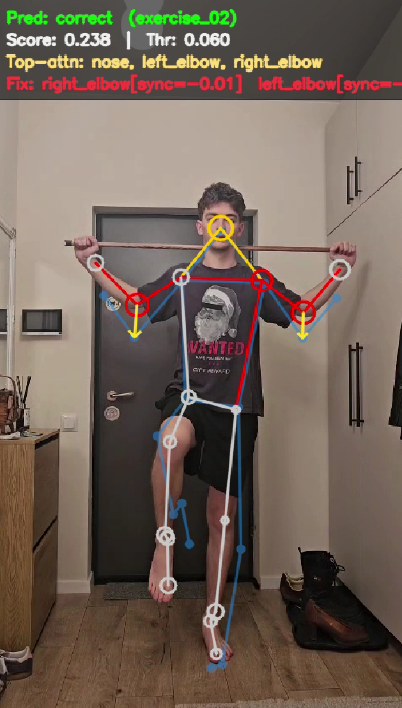
\includegraphics[width=\linewidth]{figures/ex02_start.png}
        \vspace{0.2cm} % Adds a tiny bit of space between image and text
        
        \small (a) Starting point of the movement
    \end{minipage}
    \hfill
    % Second sub-figure
    \begin{minipage}[t]{0.48\textwidth}
        \centering
        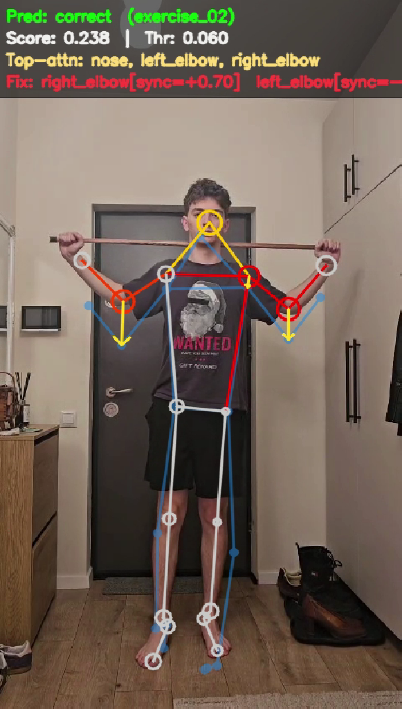
\includegraphics[width=\linewidth]{figures/ex02_halfway.png}
        \vspace{0.2cm}
        
        \small (b) Halfway through the movement
    \end{minipage}
    
    % Main figure caption
    \vspace{0.4cm} % Adds space before the main caption
    \caption{Example Annotated Video with 2 skeleton overlays: blue for the template skeleton and white/yellow/red for the MediaPipe skeleton, with corresponding colors for the worst joints.}
    \label{fig:annotated-video}
\end{figure}

\subsection{End-to-End Clinical Feedback Walkthrough}
To demonstrate the practical utility of the KinetoCheck pipeline, it is useful to examine the exact system behavior and data artifacts generated during a single rehabilitation session. Consider a scenario where a user uploads a video using the "System auto detect" feature. In this specific case, the user attempts Exercise 01 but executes it incorrectly.
\begin{figure}[H]
\centering
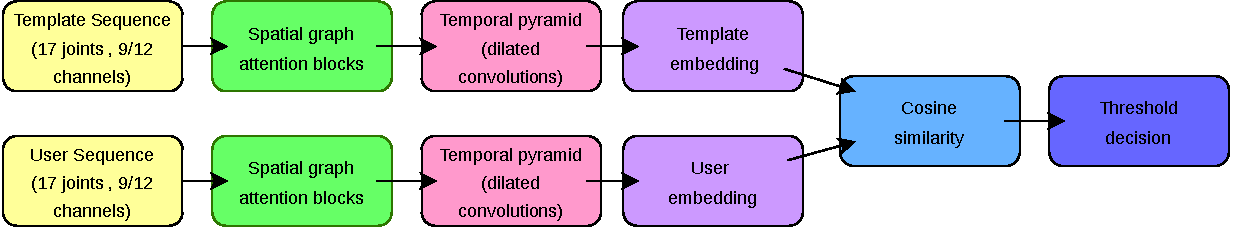
\includegraphics[width=1\textwidth]{figures/Siamese_ST-GAT.pdf}
\caption{Siamese ST-GAT with temporal pyramid architecture used in the thesis.}
\label{fig:siamese-stgat-architecture}
\end{figure}

The baseline model doesn't expose the correct skeleton execution, while the phase-aware variant provides additional metadata that improves the interpretability of the feedback.

\begin{figure}[H]
    \centering
    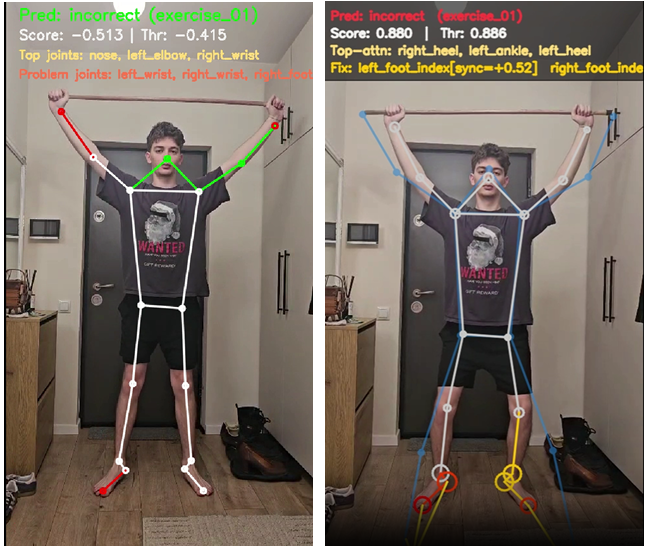
\includegraphics[width=1\textwidth]{figures/feedback_comparison.png}
    \caption{Example feedback visualizations: baseline (left) vs phase-aware (right).}
    \label{fig:feedback-comparison}
\end{figure}
Upon processing the video, the inference engine evaluates the 12-channel kinematic sequence against all ten exercise-specific ST-GAT models concurrently. Each model computes its own similarity score and compares it against its calibrated decision threshold. The system then ranks the outputs based on the classification margin (the distance between the score and the threshold). The engine packages these insights—along with localized joint error metrics—into a structured, machine-readable JSON report. A representation of this output payload is provided in Listing~\ref{lst:json-output}.

\begin{lstlisting}[language=java, caption=Generated JSON report showcasing multi-model auto-detection and joint-level insights., label=lst:json-output, frame=single, numbers=left]
{
  "video": ".../ex1-2-rep-inc.mp4",
  "annotated_video": ".../ex1-2-rep-inc_annotated.mp4",
  "num_frames": 236,
  "worst_joints": [
    {
      "joint": "right_elbow",
      "joint_index": 4,
      "deviation": 0.003,
      "importance": 0.457,
      "problem_score": 0.966
    },
    {
      "joint": "left_elbow",
      "joint_index": 3,
      "deviation": 0.003,
      "importance": 0.476,
      "problem_score": 0.981
    },
    { "..." : "..." }
  ],
  "best": {
    "exercise_id": 1,
    "exercise_name": "exercise_02",
    "score": 0.980,
    "threshold": 0.060,
    "margin": 0.920,
    "predicted_label": "correct"
  },
  "all": [
    {
      "exercise_name": "exercise_02",
      "score": 0.980,
      "threshold": 0.060,
      "margin": 0.920,
      "predicted_label": "correct"
    },
    {
      "exercise_name": "exercise_01",
      "score": 0.880,
      "threshold": 0.886,
      "margin": -0.006,
      "predicted_label": "incorrect"
    },
    { "..." : "..." }
  ]
}
\end{lstlisting}

As illustrated in Listing~\ref{lst:json-output}, the model does not merely return a binary pass/fail state. The \texttt{all} array reveals the multi-task evaluation: while the system identified the movement as a passing execution of Exercise 02 (yielding the highest positive margin of 0.920), it correctly flagged the execution as incorrect when evaluated strictly against the Exercise 01 template (failing the threshold by a margin of $-0.006$).

Furthermore, the payload isolates the anatomical source of the error within the \texttt{worst\_joints} array. In this execution, the left and right elbows are explicitly flagged as the primary components degrading the similarity score. The \texttt{importance} metric is derived directly from the Spatial Graph Attention (ST-GAT) weights, while the \texttt{deviation} magnitude is provided by the auxiliary Frame Decoder.

The ASP.NET web interface parses this payload, mapping the data to the \texttt{UploadStatistics} and \texttt{JointInsight} database entities. It then renders the user dashboard, overlaying the ghost skeleton on the video and drawing explicit visual attention to the failing joints. This pipeline successfully transforms complex, multi-model neural network outputs into a localized, interpretable, and highly actionable corrective cue for the patient.

\subsection{Longitudinal Patient Tracking and Analytics}
While isolated frame-by-frame feedback is critical for immediate postural correction, the ultimate goal of a physical rehabilitation platform is to quantify recovery over time. To serve both the patient and the overseeing physical therapist, KinetoCheck aggregates the \texttt{AnalysisHistoryEntry} database records into a comprehensive clinical statistics dashboard.

As shown in Figure~\ref{fig:app-statistics}, the system processes historical uploads to visualize the patient’s recovery trajectory. By aggregating metrics such as the total volume of exercises performed, the overall success rate, and a time-series plot of recent similarity scores, the platform provides objective proof of motor function improvement. Furthermore, by isolating the most frequently failing anatomical joints across all sessions, the system allows therapists to identify chronic biomechanical weaknesses and adjust the patient’s training regimen accordingly.

\begin{figure}[H]
    \centering
    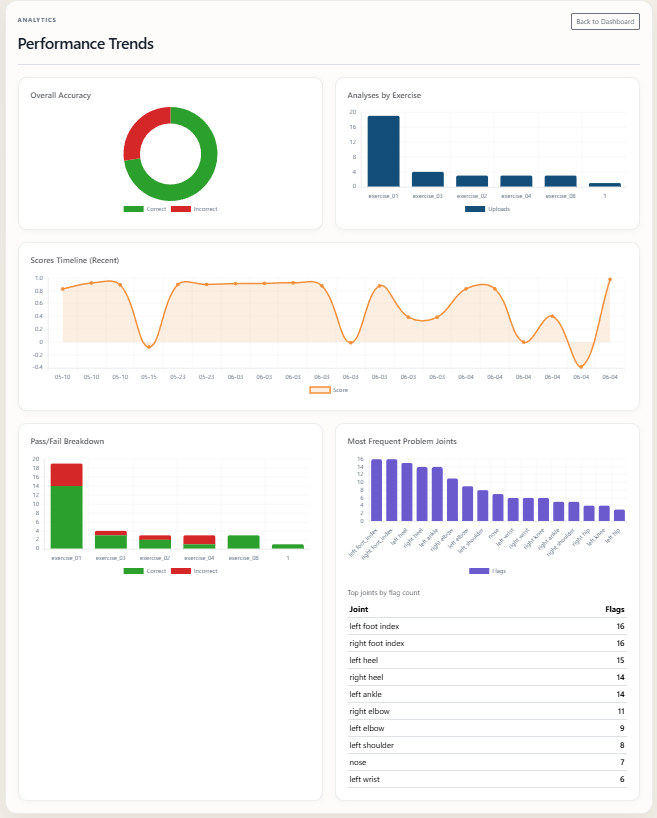
\includegraphics[width=0.85\textwidth]{figures/app_statistics.png}
    \caption{The KinetoCheck statistics dashboard, providing longitudinal analytics, success rates, and chronic joint error aggregations for long-term rehabilitation tracking.}
    \label{fig:app-statistics}
\end{figure}

\section{Generalization Challenges and Limitations}
Although results are promising, several limitations remain important to acknowledge. The primary limitation is dataset size. UI-PRMD contains 1,980 sequences across 10 subjects and 10 exercises, which is modest compared to large-scale action recognition benchmarks.

As discussed in Chapter 2, attention-based explanations should be interpreted cautiously. High attention does not automatically imply causal biomechanical error. The feedback overlays provide a useful heuristic but are not a substitute for expert clinical judgment.

\subsection{Error Analysis and Known Failure Modes}
While quantitative metrics show high performance, error analysis reveals specific edge cases where the pipeline struggles. Understanding these is critical for safe clinical deployment. The primary failure modes include:

\begin{itemize}
    \item \textbf{Severe Self-Occlusion:} During deep rotation or limb crossing, MediaPipe may lose track of distal joints. While short dropouts ($< 2$ frames) are forward-filled, extended occlusions freeze joint coordinates. The ST-GAT model interprets this rigidity as a biomechanical error, triggering false positives.
    \item \textbf{Depth Ambiguity in 2D Projections:} Extracting 3D coordinates from 2D RGB causes depth compression for movements parallel to the camera axis. The resulting drop in Z-coordinate variance can cause the model to underestimate Range of Motion (ROM) and penalize correct executions.
    \item \textbf{Clothing-Induced Landmark Jitter:} Loose clothing can confuse pose extraction, causing rapid landmark jitter. Despite Gaussian temporal smoothing, extreme high-frequency jitter is sometimes encoded by short-term convolutional kernels (\texttt{kernel size=3}) as instability, negatively skewing the similarity score.
\end{itemize}

These failure modes underscore the necessity of "Joints of Attention" overlays. Visualizing the ghost skeleton and highlighting problematic joints allows users to immediately recognize if a low score stems from genuine form error or a temporary pose-extraction failure.